\documentclass[11pt]{article}

\pagenumbering{gobble} 
\usepackage[a4paper,left=3cm, right=3cm, top=1cm, bottom=1.2cm]{geometry}
\renewcommand{\baselinestretch}{1.2}  % DEPOIS MUDAR PARA A TESE
\usepackage{hyperref}
\usepackage{graphicx}
\usepackage{caption}
\usepackage{fontspec}
\usepackage{multirow}  % table
\usepackage[table]{xcolor}  % table
%\usepackage{fancyhdr}
\usepackage{xpatch}  % table
\usepackage{tabu}  % table
\newcommand\BibTeX{B{\sc ib}\TeX}

\begin{document}

% ----------------------------------------------------> HEADER

\begingroup

\renewcommand{\baselinestretch}{1.9}
\setmainfont[Path = fonts/]{arial_narrow.ttf} 

\centering{\fontsize{12.2}{14.4}\selectfont UNIVERSIDADE DE LISBOA}\\
\centering{\fontsize{12.2}{14.4}\selectfont FACULDADE DE CIÊNCIAS}\\
\centering{\fontsize{12.2}{14.4}\selectfont DEPARTAMENTO DE BIOLOGIA ANIMAL}

\vspace{1.3cm}

\begin{figure}[h]
 \centering
 
\includegraphics[width = 6.99cm,height = 3.3cm]{images/logo.png}
\end{figure}

\vspace{3.45cm}

\setmainfont[Path = fonts/]{arial_narrow_bold.ttf}

\centering{\fontsize{17}{20.4}\selectfont Extracting Phenotype-Gene Relations
from Biomedical Literature Using Distant Supervision and Deep Learning}

\setmainfont[Path = fonts/]{arial_narrow.ttf}

\vspace{4cm}

\centering{\fontsize{14}{16.8}\selectfont Diana Francisco de Sousa}

\vspace{1.3cm}

\setmainfont[Path = fonts/]{arial_narrow_bold.ttf}

\centering{\fontsize{13}{15.6}\selectfont Mestrado em Bioinformática e Biologia Computacional}\\

\setmainfont[Path = fonts/]{arial_narrow.ttf}

%\centering{\fontsize{13}{15.6}\selectfont Especialização em Bioinformática}

\vspace{0.5cm}

\centering{\fontsize{11}{13.2}\selectfont Projeto em Bioinformática e Biologia Computacional }

\vspace{0.5cm}

\centering{\fontsize{13}{15.6}\selectfont Dissertação orientada por:}\\
\centering{\fontsize{13}{15.6}\selectfont Professor Doutor Francisco José Moreira Couto}

\vspace{2.9cm}

\centering{\fontsize{14}{16.8}\selectfont 2019}


\endgroup

\newgeometry{left=2.5cm,right=2.5cm,top=2.5cm,bottom=2.5cm}
\pagenumbering{arabic}
\setmainfont{Times New Roman}

% ----------------------------------------------------> ABSTRACT

\vspace{1cm}

\textbf{Abstract.} Identifying human phenotype-gene relations is fundamental to fully understand the origin of some phenotypic abnormalities and their associated diseases. The main comprehensive source for these relations is biomedical literature. Several relation extraction tools have been proposed to identify relations between concepts in unstructured text, namely using distant supervision and deep learning algorithms. However, most of these tools require an annotated corpus, and there is no corpus available annotated with human phenotype-gene relations. This work aims to create a human phenotype-gene relations corpus and a system that can identify them using distant supervision and deep learning algorithms. Some of the preliminary results regarding the corpus creation show a value of 87.58\% in precision, obtained from the manual evaluation by eight curators; and with deep learning algorithms a value of 70.24\% in precision in labeling a relation \textit{Known} or \textit{Unknown}.

% ----------------------------------------------------> INTRODUCTION

\section{Introduction}

% ------------------------------> MOTIVATION

\subsection{Motivation}

The volume of unstructured textual information available both on the World Wide Web and in institutional document repositories widely surpasses the ability of analysis by a researcher even if restring it to a clear-cut topic. When a researcher is interested in a specific subject searching for articles on that subject and retrieving relevant information is a time-consuming task.

Biomedical literature is the standard method that researchers use to share their findings mainly in the form of articles, patents and other types of written reports \cite{P99-1001}. The main challenges in transforming this unstructured information in useful, structured, information are that these documents follow different styles regarding the level of formality of the writing, number, and type of sections, among other things. Scientific articles regularly describe relations between human phenotype and gene entities. The main comprehensive source for articles on this topic is the PubMed\footnote{\url{https://www.ncbi.nlm.nih.gov/pubmed/}} platform, combining over 28 million citations from online books, life science journals, and the MEDLINE database \cite{Greenhalgh180}. 

Automatic methods for Information Extraction (IE) aim at obtaining useful information from large data-sets \cite{REVIEW}. Text mining uses IE methods to process text documents. These Natural Language Processing (NLP) systems need to be able to retrieve relevant information from unstructured text by including Named Entity Recognition (NER), Normalization, and Relation Extraction (RE) tasks, among others. NER consists of recognizing entities mentioned in the text by identifying the offset of its first and last character. These entities can include genes, proteins, phenotypic abnormalities, chemicals, species and other biomedical entities inserted in specific domains. Normalization consists of mapping the recognized entities to their knowledge base identifiers. RE consists of the identification of a relation between entities mentioned in a given document. Some of the commonly extracted biomedical relations are protein-protein interactions \cite{PROTEIN-PROTEIN}, drug-drug interactions \cite{BOLSTM} and disease-gene relationships \cite{DISEASE-GENE}. A detailed definition of these tasks will be provided in Section \hyperlink{5}{2.2.1}.

There are a few worth mention systems regarding biomedical RE \cite{N18-1080}, and that specifically focus on the extraction of phenotype-gene relations regarding different species types like plants \cite{PLANTS} and humans \cite{HUMANS}. The main problem that these systems face is a lack of specific high quality annotated corpus, mostly because this task requires not only a considerable amount of manual effort but also expertise knowledge about the topic. 

To extract relations between human phenotype and gene entities we have to start by: identifying the human phenotype and gene entities in a given text, and their relation (\textit{Known} or \textit{Unknown}). The first NER step influences the results of the second RE step. With genes, as a result of lexical features being relatively regular, many systems can successfully identify them in text \cite{BANNER}. However, human phenotype identification is still a complex task, only tackled by a handful of systems \cite{IHP}.

Automating searching for relations between biomedical concepts contributes to the development of pharmacogenomics, clinical trial screening, and adverse drug reaction identification \cite{doi:10.1093/bib/bbw001}. Connecting human phenotypes to genes will allow us to know more about the origin of some phenotypic abnormalities, their associated diseases, validate the results of new research, and even propose new experimental hypotheses. 

% ------------------------------> OBJECTIVE

\subsection{Objectives}

The fundamental challenge of contemporary genetic analysis is correlating genes to their respective phenotype. Existing systems that can be applied for identifying and extracting human phenotype-gene relations from biomedical literature are scarce and limited. The main challenges that they face are lack of annotated data-sets; retrieving phenotype entities, that are composed of multiple words, which makes name boundaries complex; and curating the identified relations. All of the aforementioned creates the need for corpus creation and the development of machine learning systems that can deal with the versatility of the gene and human phenotype entities and their relations to better identify and extract them. Thus, the main goals of this work are:

\begin{enumerate}

\item{Create a large and versatile silver standard corpus of human phenotype-gene relations;}

\item{Develop a module to a deep learning system for automatic extraction of human phenotype-gene relations taking advantage of domain-specific ontologies, like the Human Phenotype Ontology (HPO) and the Gene Ontology (GO);}

\item{Develop a module to a distant supervision system that combines a knowledge base for automatic extraction of  human phenotype-gene relations.}
\end{enumerate}

First, the proposed pipeline should be able to generate a silver standard corpus based on articles dedicated to human phenotype-gene relations, applying NER to identify and extract gene and human phenotype entities from the retrieved abstracts, normalizing these entities, identifying human phenotype-gene pairs that co-occur in the same sentence, and classify the relations retrieved for each article as \textit{Known} or \textit{Unknown} based on a gold standard relations file, provided by the HPO. Second, both machine learning systems (deep learning and distant supervision) should be able to process the articles in order to classify the relations retrieved for each article as \textit{Known} or \textit{Unknown}, and comparing the classification against a manually curated \textit{test-set}.

% ----------------------------------------------------> BACKGROUND

\hypertarget{2}{\section{Background}}

%This section is going to present the basic concepts and resources that support Machine Learning Text Mining based systems, namely, Natural Language Processing, Text Mining Primary Tasks and Learning Approaches, Evaluation Measures and Resources; as well as the current State-of-the-art of Biomedical Relation Extraction.

This section is going to present the basic concepts and resources that support Machine Learning Text Mining based systems, namely, Text Mining Primary Tasks and Learning Approaches, Evaluation Measures and Resources; as well as the current State-of-the-art of Biomedical Relation Extraction. 

% ------------------------------> NATURAL LANGUAGE PROCESSING

%\hypertarget{8}{\subsection{Natural Language Processing}}

%Natural Language Processing (NLP) is an area in computer science that aims computationally to derive meaning from unstructured text written by humans. NLP covers several techniques that are useful to aid the tasks described in Section \hyperlink{4}{2.2}. These text processing techniques have different goals and are often combined to obtain a better performance.

%\begin{itemize}

%\item{\textbf{Tokenization}: has the purpose of breaking the text into tokens to be processed individually or as a sequence. These tokens are usually words but can also be phrases, numbers and other types of elements. The most straightforward form of tokenization is breaking the input text by the whitespaces or punctuation. However, with scientific biomedical literature, that is usually descriptive and formal, we have to account for complex entities like human phenotype terms (composed of multiple words) and genes (represented by symbols). These specific entities and others with the same morphological complexity need specialized tokenization pipelines.} 

%\item{\textbf{Stemming and Lemmatization}: aims at reducing the variability of natural language by normalizing a token to its base form (stem) \cite{Manning:2008:IIR:1394399}. It can also take into account the context of the token, along with vocabulary and morphological analysis to determine the canonical form of the word (lemma). The stem can correspond only to a fragment of a word, but the lemma is always a real word. For example, the stem of the word \textit{having} is \textit{hav} and the lemma is \textit{have}.}

%\item{\textbf{Part-of-Speech Tagging}: consists of assigning each word of a sentence to the category where it belongs taking into account their context. Each word can be assigned to more than one category. This feature is useful to gain information on the role of a word in a given sentence.}

%\item{\textbf{Parse Tree}: represents the syntactic structure of a sentence. There are two different types of parse trees: constituency-based parse trees and dependency-based parse trees. The main difference between the two is that the first distinguishes between the terminal and non-terminal nodes and the second does not (all nodes are terminal). In constituency-based parse trees each node of the tree is either a \textit{root} node, a %\textit{branch} node, or a \textit{leaf} node. For each given sentence there is only one root node. The branch node connects to two or more \textit{child} nodes, and the leaf node is terminal. These leaves correspond to the lexical tokens \cite{AHO}. Dependency-based parse trees are usually simpler because contain fewer nodes. Parse trees generate structures that are used as inputs for other algorithms and are constructed based on supervised learning techniques.}

%\item{\textbf{Co-reference Resolution}: is a process that aims to identify which expressions refer to an entity in a given text. A reference can be a pronoun or other referring expressions. If there is more than one expression referring to the same entity these expressions are said to co-refer \cite{Jurafsky:2009:SLP:1214993}. This feature is of special relevance for the extraction of relations between entities.}

%\end{itemize}

% ------------------------------> TEXT MINING

\hypertarget{4}{\subsection{Text Mining}}

Text mining has become a widespread approach to identify and extract information from unstructured text \cite{10.1371/journal.pcbi.1005962}. Text mining is used to extract facts and relationships in a structured form that can be used to annotate specialized databases and to transfer knowledge between domains \cite{FLEUREN201597}. Text mining is a sub-field of data mining and data mining algorithms can be applied if the proper data representation, namely numeric vectors, is provided.

Even if in recent years text mining tools have evolved considerably in number and quality, there are still a few challenges of applying text mining to scientific biomedical literature. The main challenges are the complexity and heterogeneity of the written resources, making retrieving relevant information, i.e., relations between entities, not a trivial task.

Text Mining tools target different tasks, some of them performed by this thesis. The description of the main relevant tasks and approaches for the work developed is described in Sections \hyperlink{5}{2.2.1}, \hyperlink{6}{2.2.2}, and \hyperlink{7}{2.2.3}. 

% ----------------> PRIMARY TASKS

\hypertarget{5}{\subsubsection{Primary Tasks}}

The foundation of biomedical text mining is Named Entity Recognition (NER), Normalization, and Relation Extraction (RE) tasks. These tasks are used separately or together by text mining tools to extract relevant information from large data-sets, and can also be used to evaluate their performance.

\begin{itemize}

%\item{\textbf{Named Entity Recognition (NER)}: is an Information Extraction (IE) method that seeks to recognize and classify entities mentioned in unstructured text by identifying the offset of its first and last character. The workflow of this task passes by dividing the text in tokens (Section \hyperlink{8}{2.1}) and then labeling them into categories. Examples of classification are time and event expressions \cite{ULISBOA}; and, related to the biomedical domain, genes, proteins, phenotypic abnormalities, chemicals, species and other biomedical entities inserted in specific domains. In the case of this work, the focus is on human phenotype and gene entities.}

\item{\textbf{Named Entity Recognition (NER)}: is an Information Extraction (IE) method that seeks to recognize and classify entities mentioned in unstructured text by identifying the offset of its first and last character. The workflow of this task passes by dividing the text in tokens and then labeling them into categories. Examples of classification are time and event expressions \cite{ULISBOA}; and, related to the biomedical domain, genes, proteins, phenotypic abnormalities, chemicals, species and other biomedical entities inserted in specific domains. In the case of this work, the focus is on human phenotype and gene entities.}

\item{\textbf{Normalization}: IE method that matches an entity to a knowledge base identifier. For example, a gene can be written in multiple ways and mentioned by different names or acronyms in a text; normalization links all these different nomenclatures to one unique identifier. There are several resources dedicated to providing identifiers, among them the National Center for Biotechnology Information (NCBI)\footnote{\url{https://www.ncbi.nlm.nih.gov/}} for genes, and the Human Phenotype Ontology (HPO) for phenotypic abnormalities encountered in human diseases \cite{HPO}.}

%\item{\textbf{Relation Extraction (RE)}: IE method that identifies relations between entities (recognized manually or by NER) in a text. Tools manly consider relations by the co-occurrence of the entities in the same sentence, but some progress is being made to extend this task to the full document (taking into account a global context) \cite{Singhal2016TextMG}. Some of the commonly extracted biomedical relations are protein-protein interactions \cite{PROTEIN-PROTEIN}, drug-drug interactions \cite{BOLSTM} and disease-gene relationships \cite{DISEASE-GENE}.}

\item{\textbf{Relation Extraction (RE)}: IE method that identifies relations between entities (recognized manually or by NER) in a text. Tools manly consider relations by the co-occurrence of the entities in the same sentence, but some progress is being made to extend this task to the full document (taking into account a global context) \cite{Singhal2016TextMG}.}

\end{itemize}

% ----------------> GENERAL APPROACHES

\hypertarget{6}{\subsubsection{General Approaches}}

To accomplish the above tasks, one can combine multiple approaches (more common) or follow just one. Some of the fundamental approaches that are usually incorporated in the more complex ones (Section \hyperlink{7}{2.2.3}), are Classic Statistic-based and Rule-based.

\begin{itemize}

%\item{\textbf{Classic Statistic-based}: are based on statistics that can be calculated from a large data-set \cite{Manning:1999:FSN:311445}. The most common being term frequency-inverse document frequency for topic modeling, and co-occurrence for relation extraction \cite{REVIEW}. These approaches serve as a base to develop new, more intrinsic, machine learning approaches.}

\item{\textbf{Classic Statistic-based}: are based on statistics that can be calculated from a large data-set \cite{Manning:1999:FSN:311445}. The most common being term frequency-inverse document frequency for topic modeling, and co-occurrence for relation extraction \cite{REVIEW}.}

%\item{\textbf{Ruled-based}: consists of creating a set of rules using dictionaries and lists of terms, regular expressions or sentence structure that aim to extract the intent information. This approach is time-consuming and domain-specific, making it difficult to apply to other contexts. Much as the Classic approaches, Ruled-based approaches are used by more complex machine learning approaches.}

\item{\textbf{Ruled-based}: consists of creating a set of rules using dictionaries and lists of terms, regular expressions or sentence structure that aim to extract the intent information. This approach is time-consuming and domain-specific, making it difficult to apply to other contexts.}

\end{itemize}

% ----------------> MACHINE LEARNING APPROACHES (Desenvolver esta parte)

\hypertarget{7}{\subsubsection{Machine Learning Approaches}}

%Machine Learning (ML) Text Mining approaches are frequently a combination of General Approaches (Section \hyperlink{6}{2.2.2}) with more complex algorithms. As stated before data mining algorithms can be applied if the properer data representation, namely numeric vectors, is provided. Frequently, systems that are built on these approaches perform training on a \textit{training-set} that corresponds to about 70\% of the total data-set and test on a \textit{test-set} that equals to around 30\% of the total data-set and is unseen data (by the classifier) that is going to be labeled based on the generated model. Most of the times, a \textit{validation-set} is also needed and tends to correspond to 10\% of the overall data-set.

Machine Learning (ML) Learning Approaches are frequently a combination of General Approaches (Section \hyperlink{6}{2.2.2}) with more complex algorithms. Frequently, systems that are built on these approaches perform training on a \textit{training-set} that corresponds to about 70\% of the total data-set and test on a \textit{test-set} that equals to around 30\% of the total data-set and is unseen data (by the classifier) that is going to be labeled based on the generated model. Most of the times, a \textit{validation-set} is also needed and tends to correspond to 10\% of the overall data-set. 

There are two main types of ML algorithms: Supervised ML Algorithms and Unsupervised ML Algorithms. In supervised learning, the \textit{training-set} is labeled (each instance has a corresponding label, that is used to train the classifier) and in unsupervised learning the \textit{training-set} is not labeled and the training is done by the inherent structure of the input data. In this work, both types of ML algorithms were used. The supervised ML algorithm in deep learning (recurrent neural networks (RNN)) set-up and a combination of both ML algorithms in distant supervision (weak supervision) set-up.

\begin{itemize}

\item{\textbf{Recurrent Neural Networks (RNN)}: are used to train classification models based on different features such as word embeddings, that do not need to be manually crafted. Their architecture is composed of multiple layers. Each layer is responsible for learning a different type of representation of the input data, allowing for different types of tasks to be trained using the same input data. Recently, \textbf{Long-Short-Term Memory (LSTM)} networks have been proposed to be an alternative to classic RNN \cite{Hochreiter:1997:LSM:1246443.1246450}. They constitute a type of RNN that can handle long dependencies (NLP tasks usually involve long sequences of words) \cite{BOLSTM}. LSTM, through gated architecture, accounts for the vanishing of the contribution of the gradients that occurs in classic RNN by training the weights while propagating for long sequences of words. Bidirectional LSTMs have been proposed for relation extraction, since this allows that at each step, there are two LSTM layers, reading the sentence from both directions. The output is then combined to obtain a final score.}

\item{\textbf{Distant Supervision}: heuristically assigns labels to the data in the \textit{training-set} based on a provided knowledge base. This technique considers that a pair of entities in any sentence corresponding to a knowledge base entry is likely to describe a relation between those entities. Then, combining ML algorithms, adapted to distant supervision, its possible to adequately classify the data, reducing the amount of manual effort necessary. This advantage is of particular interest to the biomedical domain, because of the lack of availability of annotated corpora \cite{10.1371/journal.pone.0171929}, and allows for a corpus of any size to be used as training data. Some of the problems of distant supervision can be addressed by using \textbf{Multi-instance learning} \cite{Dietterich:1997:SMI:249678.249682}, by considering that not all co-occurrence corresponds to a relation mention. In this way, pairs of entities are grouped in bags where at least one pair in labeled as true, without knowing if all the pairs in the same bag are true, and then trained with ML algorithms.}

\end{itemize}

% ------------------------------> EVALUATION MEASURES

\hypertarget{3}{\subsection{Evaluation Measures}}

The evaluation of Machine Learning systems is done by applying the trained models to a gold standard \textit{test-set}, manually curated or annotated by domain experts and unseen by the information extraction system. For a Relation Extraction (RE) task the gold standard \textit{test-set} should correspond to the list of pairs of entities (e.g., human phenotype-gene) that co-occur in the same sentences and their relation (\textit{Known} or \textit{Unknown}).

%To any given information extraction system is necessary to define what constitutes a positive and negative result. A correct result marked though comparison with the gold standard is defined as a True Positive (TP) if present in the output or a True Negative (TN) if not present in the output. An incorrect result marked though comparison with the gold standard can be a False Positive (FP) if not present in the gold standard but present in the output or it can be a False Negative (FP) if present in the gold standard but not in the output. These types of results are described in Table \ref{table:evaluation}.

To any given information extraction system is necessary to define what constitutes a positive and negative result. These types of results are described for a RE task in Table \ref{table:evaluation}.

\begin{table}[!ht]
\small
\captionsetup{font=small}
\renewcommand\thetable{2.1}
\caption{Types of results obtained with an information extraction system for a RE task.}
\centering
\taburulecolor{black}
\begin{tabular}{ |c|c|c| }
\hline
\rowcolor[HTML]{F5F5F5} \textbf{Annotator (Gold Standard)} & \textbf{System} & \textbf{Classification}\\
\hline
\multirow{2}{*}{Relation} & Relation & True Positive (TP) \\
\cline{2-3}
 & No Relation & False Negative (FN) \\ 
\hline
\multirow{2}{*}{No Relation} & Relation & False Positive (FP) \\
\cline{2-3}
 & No Relation & True Negative (TN) \\
 \hline
\end{tabular}
\label{table:evaluation}
\end{table}

The primary goal of a given information retrieval system is to maximize the number of TP and TN. To compare results obtained with different data-sets or different tools we have three distinct evaluation metrics: \textit{recall}, \textit{precision} and \textit{F-measure}. Precision represents how often the results are correct, recall the number of correct results identified and F-measure is a combination of both metrics to express overall performance, being the harmonic mean of precision and recall:
\begin{equation}
\small
\renewcommand\theequation{2.1}
Recall = \frac{TP}{TP + FN}
\qquad
Precision = \frac{TP}{TP + FP}
\qquad
F-measure = \frac{2\times Precision\times Recall}{Precision + Recall}
\label{equation:evaluation}
\end{equation}

It is also worth noticing the inter-curator or inter-annotator agreement metric, that is going to be used in this work to evaluate the quality of the silver standard corpus annotations. This metric is calculated thought Cohen's Kappa Coefficient (κ) \cite{doi:10.1177/001316446002000104}:
\begin{equation}
\small
\renewcommand\theequation{2.2}
\kappa = \frac{P(A) - P(E)}{1 - P(E)}
\label{equation:agreement}
\end{equation}

where \textit{P}(\textit{A}) corresponds to the percentage of agreement and \textit{P}(\textit{E}) the percentage that was expected inter-curators or inter-annotators to agree by chance.

% ------------------------------> RESOURCES

\subsection{Resources}

This section as the goal of briefly describing the resources used thought this work, Tools used for NER, the Databases and Knowledge Base accessed, and the Ontologies used.

% ----------------> Systems

\subsubsection{Named Entity Recognition Tools}

The MER tool was used \cite{MER} for the annotation of the genes and the IHP framework \cite{IHP} for the annotation of human phenotype terms.

\begin{itemize}

\item{\textbf{Identification of Human Phenotype Entities Tool (IHP)}: a NER tool, specifically created to recognize HPO entities in unstructured text. It uses Stanford CoreNLP \cite{Manning2014} for text processing and applies Conditional Random Fields trained with a rich feature set, combined with hand-crafted validation rules and a dictionary to improve the recognition of human phenotypes.}

\item{\textbf{Minimal Named-Entity Recognizer Tool (MER)}: a NER tool which given any lexicon or ontology (e.g., an OWL file) and an input text is able to return a list of recognized entities, their location, and links to their classes.}

\end{itemize}

% ----------------> DATABASES AND KNOWLEDGE BASE

\hypertarget{11}{\subsubsection{Databases and Knowledge Base}}

A database is a structured way of organizing data that can be easily accessed by any computer system. A knowledge base is a resource that aims at organizing the findings provided by the literature through a single access point \cite{10.3389/fimmu.2017.01656}.

\begin{itemize}

\item{\textbf{HUGO Gene Nomenclature Committee (HGNC)}: at the European Bioinformatics Institute\footnote{\url{http://www.genenames.org/}} is responsible for approving unique symbols and names for human loci, including protein-coding genes, ncRNA genes, and pseudogenes, with the goal of promoting clear scientific communication. All approved symbols are stored in the HGNC database.}

\item{\textbf{MEDLINE}: contains journal citations and abstracts for biomedical literature from around the world \cite{Greenhalgh180}. PubMed provides free access to MEDLINE linking to full text articles when possible.}

\item{\textbf{Human Phenotype Ontology File}: is a knowledge base
that links phenotypic abnormalities to genes based on annotations retrieved from the Online Mendelian Inheritance in Man (OMIM) database.}

\end{itemize}

% ----------------> ONTOLOGIES (Depois aprofundar mais com o paper do Gruber)

\subsubsection{Ontologies}

An ontology is a structured way of providing a common vocabulary in which shared knowledge is represented \cite{Gruber}.

\begin{itemize}

\item{\textbf{Human Phenotype Ontology (HPO)}: is responsible for providing a standardized vocabulary of phenotypic abnormalities encountered in human diseases, using biomedical literature \cite{HPO}. The goal of this ontology is to facilitate medical documents readiness and exchange of medical information between medical professionals and researchers. HPO entities are often long and descriptive, not following a specific nomenclature, making it hard to identify in unstructured text.}

\item{\textbf{Gene Ontology (GO)}: defines a universe of concepts regarding gene functions (GO terms) and their relations \cite{PMID:10802651}. The GO encompass three categories (sub-ontologies): \textit{molecular function}, \textit{cellular component}, and \textit{biological process}, and three types of relations, \textit{is a}, \textit{part of} and \textit{regulates}. As in HPO terms, GO terms are usually long and descriptive. The primary goal of this ontology is to create a dynamic controlled vocabulary that can be applied to all eukaryotes, allowing for inferences regarding gene function by connecting different organisms.}


\end{itemize}

% ------------------------------> STATE-OF-THE-ART BIOMEDICAL RELATION EXTRACTION

\subsection{State-of-the-art Biomedical Relation Extraction}

This section is going to cover some of the state-of-the-art biomedical relation systems that can be adapted to the extraction of human phenotype-gene relations.

% ----------------> CLASSIFYING RELATIONS VIA LONG SHORT-TERM MEMORY NETWORKS ALONG BIOMEDICAL ONTOLOGIES (BO-LSTM)

\subsubsection{Classifying Relations via Long Short-Term Memory Networks along Biomedical Ontologies (BO-LSTM)}

The BO-LSTM system \cite{BOLSTM} is a deep learning system that is used to extract and classify relations via long short-term memory networks along biomedical ontologies. This system was created to detect and classify drug-drug interactions, taking advantage of domain-specific ontologies, like Chemical Entities of Biological Interest (ChEBI). The BO-LSTM system represents each entity as the sequence of its ancestors in their respective ontology.

% ----------------> IDENTIFYING BIOMEDICAL RELATIONS (IBREL)

\subsubsection{Identifying Biomedical Relations (IBRel)}

IBRel is an RE system \cite{10.1371/journal.pone.0171929} built for miRNA-gene relations that is based on distantly supervised multi-instance learning. This system was successfully applied to published papers about cystic fibrosis to extract miRNA-gene relations.

% ------------------------------> METHODOLOGY

\section{Methodology}

The overall methods to accomplish the proposed objectives can be divided into three stages respective to the three main goals. The first stage is the creation of a silver standard  (generated in a fully automated manner) human phenotype-gene corpus, the second stage is the development of a deep learning system for automatic extraction of human phenotype-gene relations that takes advantage of domain-specific ontologies, and the last stage is the development of a distant supervision system that combines a knowledge base for automatic extraction of human phenotype-gene relations. The experimental design in order to achieve the proposed stages is displayed in Figure \ref{figure:methodology}.

\begin{figure}[t!]
\captionsetup{font=small}
\renewcommand\thefigure{3.1}
\centering
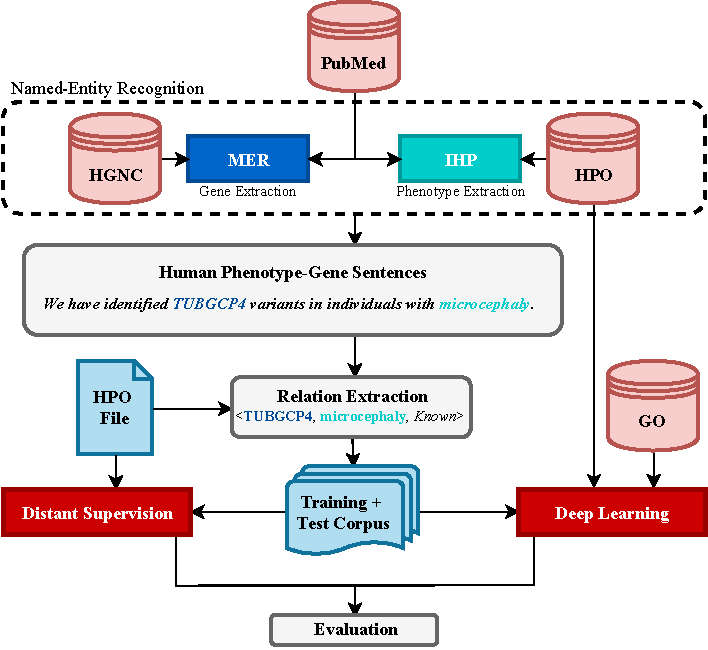
\includegraphics[width=13cm]{methods.pdf}
\fontsize{9}{10.8}\caption{Methodology overview; HUGO Gene Nomenclature Committee (\textbf{HGNC}), Minimal Named-Entity Recognizer Tool (\textbf{MER}), Identification of Human Phenotype Entities Tool (\textbf{IHP}), Human Phenotype Ontology (\textbf{HPO}), Gene Ontology (\textbf{GO}), and human phenotype-gene relations gold standard knowledge base (\textbf{HPO File}).}
\label{figure:methodology}
\end{figure}

To generate a silver standard for phenotype-gene relation extraction, we need to use a pipeline that performs: i) NER tasks, in this case, to recognize genes and human phenotype entities; ii) RE tasks, in this case, to classify a relation between human phenotype and gene entities. First, we need to gather abstracts using PubMed API with manually defined keywords, namely \textit{gene name} and \textit{homo sapiens}. Then use the MER tool \cite{MER} to extract gene mentions (the HUGO Gene Nomenclature Committee (HGNC) provided the gene terms list) in the abstracts and the IHP tool \cite{IHP} to extract human phenotype mentions (the HPO provided the human phenotype terms list). At last, use a gold standard knowledge base relations file, provided by the HPO, to classify the relations obtained by co-occurrence in the same sentence as \textit{Known} or \textit{Unknown}.

After the first stage, the corpus was divided in two sets, a \textit{training} (70\%) and a \textit{test} (30\%) set. The \textit{training} set was used to train both deep learning and distant supervision systems, the first labeled and the second unlabeled.

In the second stage, the main goal was to combine recurrent neural networks (deep learning) algorithms with biological ontologies to improve the identification of human phenotype-gene relations in biomedical literature. Ontologies such as the HPO and GO provide a reliable representation of their respective domains and can be used in order to identify those relations. The proposed system represents each entity as the sequence of its ancestors in their respective ontology and combines word embeddings and WordNet (generic English language ontology) to produce a model that can retrieve and classify the relations as \textit{Known} or \textit{Unknown}.

For the last stage, the goal was to use the unlabeled corpus generated in the first stage combined with a knowledge base (HPO File), that provides examples for the relation we wanted to extract, to apply distant supervision training. This unsupervised machine learning approach reduces the amount of manual effort necessary by discarding the annotation stage.

All three of these stages need to be evaluated. The test set was created by randomly selecting 260 relations to be reviewed by eight curators (50 relations each, with an overlap of 20 relations), all researchers working in the areas of Biology and Biochemistry. These curators had to evaluate the correctness of the classifier by attributing to each sentence one of the following options: \textit{C} (correct), \textit{I} (incorrect) or \textit{U} (uncertain). The \textit{U} option was given to identify cases of ambiguity and possible errors in the NER phase. The evaluation was done by classifying as a true positive (TP) a \textit{Known} relation that was marked \textit{C} by the curator, a false positive (FP) as a \textit{Known} relation marked \textit{I}, a false negative as a \textit{Unknown} relation marked \textit{I} and a true negative as a \textit{Unknown} relation marked \textit{C} (Section \hyperlink{3}{2.2}).

% ----------------------------------------------------> PRELIMINARY RESULTS

\section{Preliminary and Expected Results}

% ------------------------------> SILVER STANDARD CORPUS

\subsection{Silver Standard Corpus of Human Phenotype-Gene Relations Results}

\begin{itemize}

%\item{\textbf{Paper Submission}: \textit{A Silver Standard Corpus of Human Phenotype-Gene Relations} (Diana Sousa, André Lamúrias, and Francisco M. Couto) to 2019 Annual Conference of the North American Chapter of the Association for Computational Linguistics.}

\item{\textbf{Paper Submission}: \textit{A Silver Standard Corpus of Human Phenotype-Gene Relations} (Diana Sousa, André Lamúrias, and Francisco M. Couto).}

\end{itemize}

 The final results for the silver standard corpus based on articles dedicated to human phenotype-gene relations are displayed in Table \ref{table:relations}. The inter-curator agreement score, calculated from a total of 20 relations classified by eight curators, was 87.58\%. Besides the fact that there were a few incorrectly extracted relations, due to errors in the NER phase, that were discarded, the inter-curator agreement is standard.

\begin{table}[!ht]
\small
\captionsetup{font=small}
\renewcommand\thetable{4.1}
\caption{The \textit{Known} and \textit{Unknown} number of relations selected, the number of true positives, false negatives, false positives and true negatives, and the evaluation metrics for the \textit{Known} relations.} 
\linespread{1.2}\selectfont\centering
\renewcommand\arraystretch{1.4}
\taburulecolor{black}
\newcolumntype{E}{ >{\centering\arraybackslash} m{1.35cm} }
\begin{tabular}{ |c|c|E|E|E|E|c|c|c| }

\hline
\rowcolor[HTML]{F5F5F5} \multicolumn{2}{|c|}{\textbf{Relations}} & \multicolumn{4}{c|}{\textbf{Marked Relations}} & \multicolumn{3}{c|}{\textbf{Metrics}} \\
\hline
\rowcolor[HTML]{F5F5F5} \textbf{Known} & \textbf{Unknown} & \textbf{True Positive} & \textbf{False Negative} & \textbf{False Positive} & \textbf{True Negative} & \textbf{Precision} & \textbf{Recall} & \textbf{F-Measure}  \\
\hline
77 & 143 & 67 & 86 & 10 & 57 & 0.8701 & 0.4379 & 0.5826 \\
\hline
\end{tabular}
\label{table:relations}
\end{table}

The precision obtained from the test-set (about 6\% of the total of relations), was 87.01\%. Although we cannot state that this test-set is a valid representation of the overall data-set, this proves that this pipeline is a good start to automate RE corpus creation, especially between human phenotype and genes, and other domains if a gold standard relations file is provided. The lower recall is mostly due to incorrectly retrieved human phenotype annotations by IHP, that can be confirmed manually for a optimized version of the corpus, as some of them are parts of adjacent entities that can be combined for an accurate annotation. 

% ------------------------------> DEEP LEARNING SYSTEM FOR AUTOMATIC EXTRACTION OF HUMAN PHENOTYPE-GENE RELATIONS RESULTS

\subsection{Deep Learning System for Automatic Extraction of Human Phenotype-Gene Relations Results}

\begin{itemize}

\item{\textbf{Paper Published} \cite{BOLSTM}: \textit{BO-LSTM: Classifying Relations Via Long
Short-term Memory Networks Along Biomedical Ontologies.} (André Lamúrias, Diana Sousa, Luka A. Clarke, and Francisco M. Couto) to BMC Bioinformatics.}

\end{itemize}

 The model that resulted from the training of the BO-LSTM system was used to classify the relations from the test-set. The results are displayed in Table \ref{table:bolstm}. It is also showed the performance of the co-occurrence (i.e. assuming all-true) baseline method. These results are comparable to the ones obtained from the evaluation stage by the curators, and show the applicability of the corpus. The recall obtained was 0.3933. Even though this is a low number, the purpose of this work was mainly to extract correct relations between entities to facilitate ML, which was achieved by obtaining a precision of 70.24\%.
 
\begin{table}[!ht]
\small
\captionsetup{font=small}
\renewcommand\thetable{4.2}
\caption{Precision, recall and F-measure of the co-occurrence baseline and BO-LSTM methods performance.} 

\centering

\begin{tabular}{ |c|c|c|c| }

\hline
\rowcolor[HTML]{F5F5F5} \textbf{Method} & \textbf{Precision} & \textbf{Recall} & \textbf{F-Measure}\\

\hline
\cellcolor[HTML]{F5F5F5} \textbf{Co-occurrence} & 0.3231 & 1 & 0.4884 \\

\hline
\cellcolor[HTML]{F5F5F5} \textbf{BO-LSTM} & 0.7024 & 0.3933 & 0.5043 \\
	
\hline
\end{tabular}

\label{table:bolstm}
\end{table}

% ------------------------------> EXPECTED RESULTS

\subsection{Expected Results}

Based on the promising results obtained by the IBRel system \cite{10.1371/journal.pone.0171929} when applying distantly supervised multi-
instance learning combined with a knowledge base, this work expects to achieve similar results by applying analogous methods with the provided HPO knowledge base.

If possible, a new paper submission will be made to \textit{"Machine Learning and Artificial Intelligence in Bioinformatics"} journal section of BMC Bioinformatics.

Although the corpus creation pipeline can still be improved, it should be of interest to researchers working on this subject since the RE systems main problem is still a lack of annotated data-sets. Improvements may include manually correcting the 7478 human phenotype annotations extracted that did not match any HPO identifier, with the potential of expanding the number of human phenotype annotations almost 2-fold and increasing the overall recall; improving the gene extraction phase by identifying more missed gene annotations by pattern matching; expanding the corpus, which is possible due to the approach being fully automated;  using a different source to retrieve articles using the human phenotype entities as \textit{keywords} and studying the effect of different NER systems.

\section{Conclusions}

This work showed that the developed pipeline is a feasible way of creating human phenotype-gene relation corpus. Achieving promising results as shown in the manual evaluation and the BO-LSTM system application, 87.01\% and 70.24\% in precision, respectively. This work succeeded in creating a silver standard corpus with NER tools in a fully automated manner and verify its quality by manually checking a subset of annotations and by measuring the impact of using the corpus on a deep learning RE system.

% TO DELETE FOR THESIS
The general lineup of the proposed goals is displayed in Table \ref{table:tasks}.

\begin{table}[!ht]
\captionsetup{font=small}
\renewcommand\thetable{5.1}
\caption{Overview of the proposed task lineup. In blue the tasks already accomplished and in red the ones that are missing.}
\centering
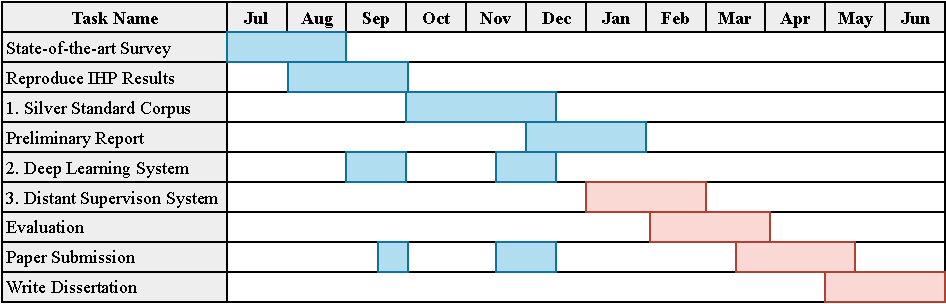
\includegraphics[width=\linewidth]{tasks.pdf}
\label{table:tasks}
\end{table}

\vspace{-10mm}
% TO DELETE FOR THESIS

\pagebreak

\bibliography{bib}
\bibliographystyle{unsrt}

\end{document}
